\section*{Naive Bayes}

Naive Bayes methods are a set of supervised learning algorithms based on applying Bayes' theorem with the "naive" assumption of conditional independence between every pair of features given the value of class variable.\\ \\
What actually Bayes' theorem is?
\begin{equation}\label {eq:bayes}
	P(A|B) = \frac{P(B|A)P(A)}{P(B)}
\end{equation}
$P(A|B)$ is the probability of \textbf{A} happening, given that \textbf{B} has occured.\\ \\ Why "Naive"? Because the presence of one particular feature does not affect the other.
\\ \\ 
Without going to deep, let's see an example:

\subsection*{The Golf Match Problem}
	Consider the problem of playing golf, dataset for the same:
	\begin{figure}[h]
		\centering
		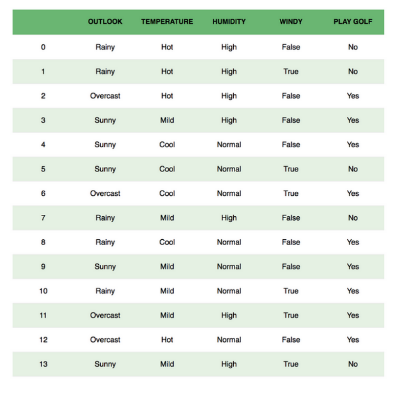
\includegraphics[scale=0.7]{golf.png}
		\caption{Dataset for possiblity of a golf match}
	\end{figure}

	Bayes theorem for this example can be rewritten as:
	\begin{equation}
		P(y|X) = \frac{P(X|y)P(y)}{P(X)}
	\end{equation}

	The variable \textbf{y} is the class variable (play golf), which represents if it is suitable to play golf or not given the conditions. Variable \textbf{X} is a matrix representing the parameters/features.
	\\ \\
	$\textbf{X} = (x_1, x_2, x_3, ... , x_n)$ \hfill	\small{$x_1, x_2, ... x_n$ represent the features}\footnote[1]{temperature, humidity and windy (here)}.
	\\ \\

	\begin{equation}
		P(y|x_1, ..., x_n) = \frac{P(x_1|y)P(x_2|y)...P(x_n|y)P(y)}{P(x_1)P(x_2)...P(x_n)}
	\end{equation}
	These values can be obtained by looking at the dataset and substituting them into equation will give us the result.
	\\ \\
	In our case, the the class variable(\textbf{y}) has only two outcomes, yes or no. Therefore, we need to find class \textbf{y} with maximum probability. 
	\begin{equation}
		y = argmax_yP(y)\prod_{i=1}^{n}P(x_i|y)
	\end{equation}

\subsection*{Types of Naive Bayes classifier:}
	\subsubsection*{Miltinomial Naive Bayes:}
		This is mostly used for document classification problem, i.e whether a document belongs to the category of sports, politics, technology etc. The features/predictors used by the classifier are the frequency of the words present in the document.

	\subsubsection*{Bernoulli Naive Bayes}
		This is similar to the multinomial naive bayes but the predictors are boolean variables. The parameters that we use to predict the class variable take up only values yes or no, for example if a word occurs in the text or not.

	\subsubsection*{Gaussian Naive Bayes}
		When the predictors take up a continuous value and are not discrete, we assume that these values are sampled from a gaussian distribution.

		\begin{figure}[h]
			\centering
			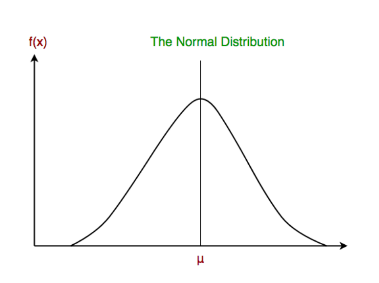
\includegraphics[scale=0.6]{gaussiannaive.png}
			\caption{Gaussian Distribution(Normal Distribution)}
		\end{figure}

		The formula for conditional probability changes to:

		\begin{equation}
			P(x_i|y) = \frac{1}{\sqrt{2\pi\sigma_y^2}}e^{-\frac{(x_i-\mu_y)^2}{2\sigma_y^2}}
		\end{equation}

\subsection*{Laplace Smoothing}
	It is problematic when a frequency-based probability is zero, because it will wipe out all the information in the other probabilities.\\ \\
	A solution would be \textbf{Laplace smoothing} , which is a technique for smoothing categorical data. A small-sample correction, or \textbf{pseudo-count}, will be incorporated in every probability estimate. Consequently, no probability will be zero. this is a way of regularizing Naive Bayes, and when the pseudo-count is zero, it is called Laplace smoothing. While in the general case it is often called \textbf{Lidstone smoothing.}

	\begin{equation}
		P_{i,\ \alpha-smoothed} = \frac{x_i+\alpha}{N+\alpha d}
	\end{equation}
	where, $\alpha > 0$ the "pseudocount" is a smoothing parameter. And, $1/d$ is the \href{https://en.wikipedia.org/wiki/Discrete_uniform_distribution}{Uniform Probability}.

	\subsubsection*{Note}
	In practice, we use logs to represent probabilities:
	\begin{equation}
		\log{(P(x_1|y)P(x_2|y)...P(x_n|y))} = \log{P(x_1|y)} + \log{P(x_2|y)} +...+ \log{P(x_n|y)}
	\end{equation}


\subsection*{Applications}
	Naive Bayes algorithms are mostly used in sentiment analysis, spam filtering, recommendation systems etc. They are fast and easy to implement but their biggest disadvantage is that the requirement of predictors to be independent. In most of the real life cases, the predictors are dependent, this hinders the performance of the classifier.

\subsection*{Worked-out Implementation}
\lstinputlisting[language=Python, caption=Python Implementation for Naive Bayes]{naiveBayes-implementation.py}
